\documentclass[a4paper,12pt]{article}

%%% Работа с русским языком % для pdfLatex
\usepackage{cmap}					% поиск в~PDF
\usepackage{mathtext} 				% русские буквы в~фомулах
\usepackage[T2A]{fontenc}			% кодировка
\usepackage[utf8]{inputenc}			% кодировка исходного текста
\usepackage[english,russian]{babel}	% локализация и переносы
\usepackage{indentfirst} 			% отступ 1 абзаца

%%% Работа с русским языком % для XeLatex
%\usepackage[english,russian]{babel}   %% загружает пакет многоязыковой вёрстки
%\usepackage{fontspec}      %% подготавливает загрузку шрифтов Open Type, True Type и др.
%\defaultfontfeatures{Ligatures={TeX},Renderer=Basic}  %% свойства шрифтов по умолчанию
%\setmainfont[Ligatures={TeX,Historic}]{Times New Roman} %% задаёт основной шрифт документа
%\setsansfont{Comic Sans MS}                    %% задаёт шрифт без засечек
%\setmonofont{Courier New}
%\usepackage{indentfirst}
%\frenchspacing

%%% Дополнительная работа с математикой
\usepackage{amsfonts,amssymb,amsthm,mathtools}
\usepackage{amsmath}
\usepackage{icomma} % "Умная" запятая: $0,2$ --- число, $0, 2$ --- перечисление
\usepackage{upgreek}

%% Номера формул
%\mathtoolsset{showonlyrefs=true} % Показывать номера только у тех формул, на которые есть \eqref{} в~тексте.

%%% Страница
\usepackage{extsizes} % Возможность сделать 14-й шрифт

%% Шрифты
\usepackage{euscript}	 % Шрифт Евклид
\usepackage{mathrsfs} % Красивый матшрифт

%% Свои команды
\DeclareMathOperator{\sgn}{\mathop{sgn}} % создание новой конанды \sgn (типо как \sin)
\usepackage{csquotes} % ещё одна штука для цитат
\newcommand{\pd}[2]{\ensuremath{\cfrac{\partial #1}{\partial #2}}} % частная производная
\newcommand{\abs}[1]{\ensuremath{\left|#1\right|}} % модуль
\renewcommand{\phi}{\ensuremath{\varphi}} % греческая фи
\newcommand{\pogk}[1]{\!\left(\cfrac{\sigma_{#1}}{#1}\right)^{\!\!\!2}\!} % для погрешностей

% Ссылки
\usepackage{color} % подключить пакет color
% выбрать цвета
\definecolor{BlueGreen}{RGB}{49,152,255}
\definecolor{Violet}{RGB}{120,80,120}
% назначить цвета при подключении hyperref
\usepackage[unicode, colorlinks, urlcolor=blue, linkcolor=blue, pagecolor=blue, citecolor=blue]{hyperref} %синие ссылки
%\usepackage[unicode, colorlinks, urlcolor=black, linkcolor=black, pagecolor=black, citecolor=black]{hyperref} % для печати (отключить верхний!)


%% Перенос знаков в~формулах (по Львовскому)
\newcommand*{\hm}[1]{#1\nobreak\discretionary{}
	{\hbox{$\mathsurround=0pt #1$}}{}}

%%% Работа с картинками
\usepackage{graphicx}  % Для вставки рисунков
\graphicspath{{images/}{images2/}}  % папки с картинками
\setlength\fboxsep{3pt} % Отступ рамки \fbox{} от рисунка
\setlength\fboxrule{1pt} % Толщина линий рамки \fbox{}
\usepackage{wrapfig} % Обтекание рисунков и таблиц текстом
\usepackage{multicol}

%%% Работа с таблицами
\usepackage{array,tabularx,tabulary,booktabs} % Дополнительная работа с таблицами
\usepackage{longtable}  % Длинные таблицы
\usepackage{multirow} % Слияние строк в~таблице
\usepackage{caption}
\captionsetup{labelsep=period, labelfont=bf}

%%% Оформление
\usepackage{indentfirst} % Красная строка
%\setlength{\parskip}{0.3cm} % отступы между абзацами
%%% Название разделов
\usepackage{titlesec}
\titlelabel{\thetitle.\quad}
\renewcommand{\figurename}{\textbf{Рис.}}		%Чтобы вместо figure под рисунками писал "рис"
\renewcommand{\tablename}{\textbf{Таблица}}		%Чтобы вместо table над таблицами писал Таблица

%%% Теоремы
\theoremstyle{plain} % Это стиль по умолчанию, его можно не переопределять.
\newtheorem{theorem}{Теорема}[section]
\newtheorem{proposition}[theorem]{Утверждение}

\theoremstyle{definition} % "Определение"
\newtheorem{definition}{Определение}[section]
\newtheorem{corollary}{Следствие}[theorem]
\newtheorem{problem}{Задача}[section]

\theoremstyle{remark} % "Примечание"
\newtheorem*{nonum}{Решение}
\newtheorem{zamech}{Замечание}[theorem]

%%% Правильные мат. символы для русского языка
\renewcommand{\epsilon}{\ensuremath{\varepsilon}}
\renewcommand{\phi}{\ensuremath{\varphi}}
\renewcommand{\kappa}{\ensuremath{\varkappa}}
\renewcommand{\le}{\ensuremath{\leqslant}}
\renewcommand{\leq}{\ensuremath{\leqslant}}
\renewcommand{\ge}{\ensuremath{\geqslant}}
\renewcommand{\geq}{\ensuremath{\geqslant}}
\renewcommand{\emptyset}{\varnothing}

%%% Для лекций по инфе
\usepackage{tikz}  
\usetikzlibrary{graphs}
\usepackage{alltt}
\newcounter{infa}[section]
\newcounter{num}
\definecolor{infa}{rgb}{0, 0.2, 0.89}
\definecolor{infa1}{rgb}{0, 0.3, 1}
\definecolor{grey}{rgb}{0.5, 0.5, 0.5}
\newcommand{\tab}{\ \ \ }
\newcommand{\com}[1]{{\color{grey}\# #1}}
\newcommand{\num}{\addtocounter{num}{1}\arabic{num}\tab}
\newcommand{\defi}{{\color{infa}def}}
\newcommand{\globali}{{\color{infa}global}}
\newcommand{\ini}{{\color{infa}in}}
\newcommand{\rangei}{{\color{infa}range}}
\newcommand{\fori}{{\color{infa}for}}
\newcommand{\ifi}{{\color{infa}if}}
\newcommand{\elsei}{{\color{infa}else}}
\newcommand{\printi}{{\color{infa1}print}}
\newcommand{\enumeratei}{{\color{infa1}enumerate}}
\newcommand{\maxi}{{\color{infa}max}}
\newcommand{\classi}{{\color{infa}class}}
\newcommand{\returni}{{\color{infa}return}}
\newcommand{\elifi}{{\color{infa}elif}}
\newcommand{\seti}{{\color{infa}set}}
\newcommand{\noti}{{\color{infa}not}}
\newcommand{\dicti}{{\color{infa}dict}}
\newcommand{\zipi}{{\color{infa}zip}}
\newcommand{\chri}{{\color{infa}chr}}
\newcommand{\ordi}{{\color{infa}ord}}
\newcommand{\leni}{{\color{infa}len}}
\newcommand{\deli}{{\color{infa}del}}
\newcommand{\sortedi}{{\color{infa}sorted}}
\newcommand{\keyi}{{\color{infa}key}}
\newcommand{\lambdai}{{\color{infa}lambda}}
\newcommand{\inti}{{\color{infa}int}}
\newcommand{\inputi}{{\color{infa}input}}
\newcommand{\isi}{{\color{infa}is}}
\newcommand{\Nonei}{{\color{infa}None}}
\newcommand{\whilei}{{\color{infa}while}}
\newcommand{\andi}{{\color{infa}and}}
\newcommand{\fromi}{{\color{infa}from}}
\newcommand{\importi}{{\color{infa}import}}
\newcommand{\continuei}{{\color{infa}continue}}
\newcommand{\mapi}{{\color{infa}map}}
\newcommand{\Falsei}{{\color{infa1}False}}
\newcommand{\listi}{{\color{infa}list}}
\newcommand{\Truei}{{\color{infa1}True}}
\newcommand{\mini}{{\color{infa1}min}}


\newenvironment{infa}[1]{
	
	\vspace{0.5cm}
	\addtocounter{infa}{1}%
	\noindent{\large \textbf{Программа №\thesection.\arabic{infa}.}\ \textbf{#1}}%
	\begin{alltt}%
	}{\end{alltt}
	\setcounter{num}{0}
	\vspace{0.1cm}}
\newenvironment{infanoname}{
	
	%\vspace{0.5cm}
	%\addtocounter{infa}{1}%
	%\noindent{\large \textbf{Программа №\thesection.\arabic{infa}.}\ \textbf{#1}}%
	\begin{alltt}%
	}{\end{alltt}
	\setcounter{num}{0}
	\vspace{0.1cm}}

\usepackage{animate} % Для добавления гифок
\usepackage{xmpmulti}
%Пример кода:
%\begin{infa}{Поразрядная сортировка}
%	\ \num \defi count_sort(a):\tab \com{определяет нашу функцию}
%	\ \num \tab m = \maxi(a)+1
%	\ \num \tab q = [0]*m
%	\ \num \tab \fori x \ini a:
%	\ \num \tab \tab q[x] += 1
%	\ \num \tab pos = 0
%	\ \num \tab \fori x \ini q:
%	\ \num \tab \tab \fori i \ini \rangei(q[x]):
%	\ \num \tab \tab \tab a[pos] = x
%	\num \tab \tab \tab pos += 1
%\end{infa}

\usepackage[left=1.27cm,right=1.27cm,top=1.27cm,bottom=2cm]{geometry}
%\hbox to\textwidth{команда колонтитула}
\begin{document}
\newcounter{lec}
\newcommand{\lec}[1]{\addtocounter{lec}{1} \setcounter{section}{0}%
\begin{center}
{\LARGE ЛЕКЦИЯ \arabic{lec}%
\vspace{2mm}%

\textbf{#1}%
}
\end{center}
}
\newpage
\
\setcounter{lec}{5}
\lec{}
\section{Алгоритм Флойда-Уоршела}
\subsection{Описание алгоритма}
\textbf{Задача алгоритма:} \emph{нахождение кратчайших расстояний между всеми вершинами взвешенного ориентированного графа.}

Алгоритм: на каждом шаге проверяем новое количество вершин, т.е. на первом шаге имеем путь между двумя соседними вершинами --- ребро, соединяющее вершины. На втором шаге выбираем какую-то вершину и смотрим, будет ли короче путь между двумя изначальными вершинами, если пройти через эту выбранную точку. Далее выбираем следующую точку и т.д. Таким образом мы постепенно исследуем все пути из вершины в вершину через постепенно растущее число вершин. 

Строим последовательность матриц (методом динамического программирования) $a_{ij}^0 \rightarrow a^1_{ij} \rightarrow a^2_{ij} \rightarrow\dots\rightarrow a^n_{ij}$. $a^k_{ij}$ --- кратчайшее расстояние от i-ой до j-ой вершины, при этом как промежуточными пользуемся от 1-ой до k-ой.\\
$a_{ij}^0 = W_{ij}$ --- промежуточными вершинами пользоваться нельзя.\\
Правило поиска следующей матрицы: $a_{ij}^k= \min(a^{k-1}_{ij}, a^{k-1}_{ik}+a^{k-1}_{kj}).$\\
Сложность алгоритма: $O(N^3)$.

Более подробно алгоритм описан в \href{https://ru.wikipedia.org/wiki/%D0%90%D0%BB%D0%B3%D0%BE%D1%80%D0%B8%D1%82%D0%BC_%D0%A4%D0%BB%D0%BE%D0%B9%D0%B4%D0%B0_%E2%80%94_%D0%A3%D0%BE%D1%80%D1%88%D0%B5%D0%BB%D0%BB%D0%B0}{википедии}.
\subsection{Реализация}
Будем запоминать все предыдущие матрицы (что необязательно).

\begin{infa}{Реализация алгоритма Флойда-Уоршела}
\num A = [[[INF]*n \fori i \ini \rangei(n)] \fori k \ini \rangei(n+1)] \com{INF - условная\\\phantom{6\ \ \ \ }бесконечность, n - число ребер}
\num \fori i \ini \rangei(n):
\num \tab A[0][i][:] = W[i] \com{При копировании весовой матрицы W расстояние от вершины\\\phantom{6\ \ \ \ }до себя равно нулю; забиваем матрицу рёбер т.е. расстояния в начальный момент.}
\num \fori k \ini \rangei(1, n+1):
\num \tab \fori i \ini \rangei(n):
\num \tab \tab \fori j \ini \rangei(n):
\num \tab \tab \tab A[k][i][j] = \mini(A[k-1][i][j], A[k-1][i][k]+A[k-1][k][j]) \com{Добав-\\\phantom{6\ \ \ \ }ляем путь от i до j вершины через новую вершину, если такой путь короче}
\end{infa}
Алгоритм не работает с циклами отрицательного веса, т.к. можно <<накрутить>> минус бесконечность. Но если при этом путь от i-ой до j-ой вершины не содержит такого цикла, то алгоритм сработает правильно.
\section{Топологическая сортировка}
Если граф не содержит циклов, то его вершины можно пронумеровать так, что любое ребро идет от вершины с меньшим номером к вершине с большим номером.

\textsf{Топологическая сортировка} — упорядочивание вершин бесконтурного ориентированного графа согласно частичному порядку, заданному ребрами орграфа на множестве его вершин.

Т.е. если граф не содержит циклов, то его вершины можно пронумеровать так, что любое ребро идет от вершины с меньшим номером к вершине с большим номером.\\
Применяется в различных прикладных задачах. 

\subsection{Алгоритм Кана}
\noindent A(k) --- множество вершин, от которых <<зависит>> вершина k (т.е. в которую можно прийти от других вершин).\\P --- последовательность вершин.\\
Алгоритм:\\
\texttt{Пока \abs{P} < N:\\
\phantom{\tab }Найти вершину v, у которой A(v) = $\varnothing$ \\%пустое множество
\phantom{\tab }P.append(v)\\
\phantom{\tab }Вычеркнуть v из всех множеств A(k).\\}
Алгоритм очень громоздкий и неэффективный.
\subsection{Алгоритм Тарьяна}
\subsubsection{Алгоритм}
Сложность алгоритма: $O(n)$.\\
По факту мы просто осуществляем обход в глубину, в котором мы будем красить вершины.\\
\textsf{Подход алгоритма:} DFS с покраской вершин (белая/серая/черная).\\
С любой вершины не used вершины запускаем DFS. Белые вершины --- еще не тронутые, серые вершины --- те, в которые алгоритм вошел, черные вершины --- те, из которого алгоритм вышел.\\
Попытка входа в серую вершины означает наличие цикла, значит алгоритм невозможен.
При выходе из вершины (в момент покраски ее в черный цвет) добавляем ее в начало списка.

\subsubsection{Реализация алгоритма}
\begin{infa}{Реализация алгоритма Тарьяна}
	\ \num Visited = [\Falsei]*(n + 1)
	\ \num Ans = []
	\ \num 
	\ \num \defi DFS(start):
	\ \num \tab Visited[start] = \Truei
	\ \num \tab \fori u \ini V[start]:
	\ \num \tab \tab \ifi \noti Visited[u]:
	\ \num \tab \tab \tab DFS(u)
	\ \num \tab Ans.append(start)
	\num
	\num \fori i \ini \rangei(1, n + 1): 
	\num \tab \ifi \noti Visited(i): 
	\num \tab \tab DFS(i) 
	\num Ans = Ans[::-1]
\end{infa}
%рисунок 2
%реализации не будет
\section{Неэффективные алгоритмы}
\subsection{Задача Коммивояжера}
\textbf{Задача:} \emph{найти минимальный по весу гамильтонов цикл. Сложность алгоритма: $O(N!)$.}

В графе есть вершины. Коммивояжер захотел посетить  все эти вершины и вернутся домой. Гамильтонов цикл точно есть в этой системе (это легко проверить, соединив все вершины по порядку). То есть, задача сводится к тому, чтобы найти минимальный по весу Гамильтонов цикл. Но эта задача плохо реализуется при большом числе вершин, так как основа решения --- перебор. Т.е. имеем $N!$ потенциально возможных гамильтоновых циклов, каждый имеет свой вес.

К примеру, на рис. \ref{ris1} изображен оптимальный маршрут коммивояжёра через 15 крупнейших городов Германии. Указанный маршрут является самым коротким из всех возможных 43 589 145 600 вариантов.
\begin{figure}[h!]
	\centering
	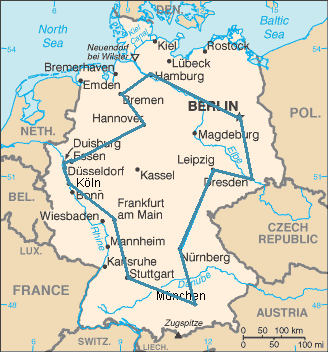
\includegraphics[width=0.5\linewidth]{germany}
	\caption{Оптимальный маршрут коммивояжёра через 15 крупнейших городов Германии}
	\label{ris1}
\end{figure}

Таким образом оптимизировать эту задачу невозможно.

%рис 3, нужно доехать из A в B и посетить все пункты
\subsection{Задача о китайском почтальоне}
%рис 4
\textbf{Задача:} \emph{пройти по каждому ребру графа минимум 1 раз, чтобы доставить почту. Требуется найти такой цикл минимального суммарного веса.}

То есть, нам необходимо найти цикл минимального суммарного веса, такой, что он проходит по ребру хотя бы 1 раз. Важное замечание --- если граф Эйлеров, то Эйлеров цикл и есть решение этой задачи. А вот если его нет, то задача усложняется --- решение можно найти только полным перебором. Итоговый алгоритм получается неэффективным, т.к. его асимптотика $O(N!)$.










\begin{center}
	\vfill \emph{{\small Г. С. Демьянов, \href{https://vk.com/id37346992}{VK}\\
С. С. Клявинек, \href{https://vk.com/id85132547}{VK}
}}
\end{center}






\end{document} 